
%% Friction Questions used on the
%% NYSED Physics Regents Examination
%%--------------------------------------------------

%% this section contains 40 problems


%% Section June2016
%%--------------------
\element{nysed}{
\begin{question}{June2016-Q03}
    When the sum of all the forces acting on a block on an inclined plane is zero, the block:
    \begin{choices}
        \wrongchoice{must be at rest}
        \wrongchoice{must be accelerating}
        \wrongchoice{may be slowing down}
      \correctchoice{may be moving at constant speed}
    \end{choices}
\end{question}
}

\element{nysed}{
\begin{question}{June2016-Q39}
    A box weighing \SI{46}{\newton} rests on an incline that makes an angle of \ang{25} with the horizontal.
    What is the magnitude of the component of the box's weight perpendicular to the incline?
    \begin{multicols}{2}
    \begin{choices}
        \wrongchoice{\SI{19}{\newton}}
        \wrongchoice{\SI{21}{\newton}}
      \correctchoice{\SI{42}{\newton}}
        \wrongchoice{\SI{46}{\newton}}
    \end{choices}
    \end{multicols}
\end{question}
}


%% Section June2015
%%--------------------


%% Section June2014
%%--------------------


%% Section June2013
%%--------------------
\element{nysed}{
\begin{question}{June2013-Q08}
    An \SI{8.0}{\newton} wooden block slides across a horizontal wooden floor at constant velocity.
    What is the magnitude of the force of kinetic friction between the block and the floor?
    %% NOTE: Requies reference to NYSED reference sheet
    \begin{multicols}{2}
    \begin{choices}
      \correctchoice{\SI{2.4}{\newton}}
        \wrongchoice{\SI{3.4}{\newton}}
        \wrongchoice{\SI{8.0}{\newton}}
        \wrongchoice{\SI{27}{\newton}}
    \end{choices}
    \end{multicols}
\end{question}
}

\element{nysed}{
\begin{question}{June2013-Q12}
    An \SI{8.0}{\newton} block is accelerating down a frictionless ramp inclined at \ang{15} to the horizontal,
        as shown in the diagram below.
    \begin{center}\small
    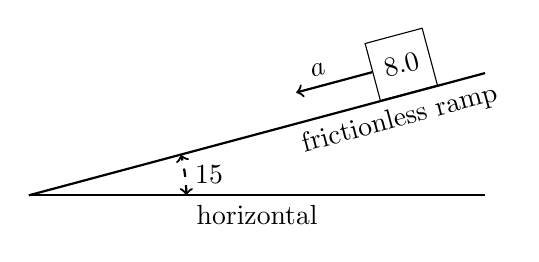
\begin{tikzpicture}
        %% Ramp
        \draw[thick] (0,0) -- (15:6)
            node[pos=0.80,anchor=north,rotate=15] {frictionless ramp};
        \draw[thick,<->,dashed] (0:2) arc (0:15:2)
            node[pos=0.5,anchor=west] {\ang{15}};
        %% Block
        \node[draw,rectangle,minimum size=0.75cm,rotate=15,anchor=south]
            (B) at (15:5) {\SI{8.0}{\newton}};
        \draw[thick,->] (B.west) -- ++ (195:1) node[pos=0.66,anchor=south,rotate=15] {$a$};
        %% Horizontal
        \draw[thick] (0:0) -- (0:5.8)
            node[pos=0.5,anchor=north] {horizontal};
    \end{tikzpicture}
    \end{center}
    What is the magnitude of the net force causing the block's acceleration?
    \begin{multicols}{2}
    \begin{choices}
        \wrongchoice{\SI{0}{\newton}}
      \correctchoice{\SI{2.1}{\newton}}
        \wrongchoice{\SI{7.7}{\newton}}
        \wrongchoice{\SI{8.0}{\newton}}
    \end{choices}
    \end{multicols}
\end{question}
}


%% Section June2012
%%--------------------
\element{nysed}{
\begin{question}{June2012-Q11}
    A \SI{0.50}{\kilo\gram} puck sliding on a horizontal shuffleboard court is slowed to rest by a frictional force of \SI{1.2}{\newton}.
    What is the coefficient of kinetic friction between the puck and the surface of the shuffleboard court?
    \begin{multicols}{2}
    \begin{choices}
      \correctchoice{\num{0.24}}
        \wrongchoice{\num{0.42}}
        \wrongchoice{\num{0.60}}
        \wrongchoice{\num{4.1}}
    \end{choices}
    \end{multicols}
\end{question}
}


%% Section June2011
%%--------------------
\element{nysed}{
\begin{question}{June2011-Q39}
    A child pulls a wagon at a constant velocity along a level sidewalk.
    The child does this by applying a \SI{22}{\newton} force to the wagon handle,
        which is inclined at \ang{35} to the sidewalk as shown below.
    \begin{center}
    \begin{tikzpicture}
        %% ground
        \draw (-4,0) -- (4,0);
        \node[anchor=north,minimum width=8cm,pattern=north east lines] at (0,0) {};
        \node[anchor=north] at (0,-1em) {Level sidewalk};
        %% Cart
        \node[draw,fill=white!90!black,minimum height=1.33cm,minimum width=2cm,anchor=south] (L) at (-1,0.33) {};
        \draw[fill=white] (L.south west) ++(0:0.5) circle (0.33);
        \draw[fill=black] (L.south west) ++(0:0.5) circle (1pt);
        \draw[fill=white] (L.south east) ++(180:0.5) circle (0.33);
        \draw[fill=black] (L.south east) ++(180:0.5) circle (1pt);
        %% vector
        \draw[thick,->] (L.east) -- ++(35:3) node[pos=0.5,anchor=south,rotate=35] {\SI{22}{\newton}};
        \draw[dashed] (L.east) -- ++(0:{3*cos(35)});
        \draw (L.east) ++ (0:1.5) arc(0:35:1.5) node[pos=0.5,anchor=west] {\ang{35}};
    \end{tikzpicture}
    \end{center}
    What is the magnitude of the force of friction on the wagon?
    \begin{multicols}{2}
    \begin{choices}
        \wrongchoice{\SI{11}{\newton}}
        \wrongchoice{\SI{13}{\newton}}
      \correctchoice{\SI{18}{\newton}}
        \wrongchoice{\SI{22}{\newton}}
    \end{choices}
    \end{multicols}
\end{question}
}


%% Section June2010
%%--------------------


%% Section June2009
%%--------------------


%% Section Jan2009
%%--------------------
\element{nysed}{
\begin{question}{Jan2009-Q11}
    Which statement best explains why a ``wet saw'' used to cut through fine optical crystals is constantly lubricated with oil?
    \begin{choices}
      \correctchoice{Lubrication decreases friction and minimizes the increase of internal energy.}
        \wrongchoice{Lubrication decreases friction and maximizes the increase of internal energy.}
        \wrongchoice{Lubrication increases friction and minimizes the increase of internal energy.}
        \wrongchoice{Lubrication increases friction and maximizes the increase of internal energy.}
    \end{choices}
\end{question}
}

\element{nysed}{
\begin{question}{Jan2009-Q37}
    The diagram below shows a \SI{1.0e5}{\newton} truck at rest on a hill that makes an angle of \ang{8.0} with the horizontal.
    \begin{center}
    \pgfdeclarelayer{bg}
    \pgfsetlayers{bg,main}
    \begin{tikzpicture}
        %% incline
        \draw[thick] ({8*cos(8)},0) -- (0,0) -- (8:8);
        \node[anchor=north] at (4,0)  {Horizontal};
        \draw[<->] (6,0) arc (0:8:6) node[pos=0.5,anchor=west] {\ang{8.0}};
        %% Truck
        \begin{pgfonlayer}{main}
            \node[draw,fill=white,minimum size=0.1cm,circle,rotate=8,anchor=south] (W1) at (8:2.5) {};
            \node[draw,fill=white,minimum size=0.1cm,circle,rotate=8,anchor=south] (W2) at (8:3.05) {};
            \node[draw,fill=white,minimum size=0.1cm,circle,rotate=8,anchor=south] (W3) at (8:4.1) {};
            \draw[fill=white!60!black] (W1) circle (1pt);
            \draw[fill=white!60!black] (W2) circle (1pt);
            \draw[fill=white!60!black] (W3) circle (1pt);
        \end{pgfonlayer}
        \begin{pgfonlayer}{bg}
            \node[draw,minimum size=0.5cm,anchor=south,rotate=8,shift={(105:-0.2)}] (R) at (W1.north) {};
            \node[draw,minimum width=1.5cm,minimum height=0.8cm,anchor=south west,rotate=8] at (R.south east) {\SI{e5}{\newton}};
        \end{pgfonlayer}
    \end{tikzpicture}
    \end{center}
    What is the component of the truck’s weight parallel to the hill?
    \begin{multicols}{2}
    \begin{choices}
        \wrongchoice{\SI{1.4e3}{\newton}}
        \wrongchoice{\SI{1.0e4}{\newton}}
      \correctchoice{\SI{1.4e4}{\newton}}
        \wrongchoice{\SI{9.9e4}{\newton}}
    \end{choices}
    \end{multicols}
\end{question}
}


%% Section June2008
%%--------------------
\element{nysed}{
\begin{question}{June2008-Q08}
    A \SI{1200}{\kilo\gram} space vehicle travels at \SI{4.8}{\meter\per\second} along the level surface of Mars.
    If the magnitude of the gravitational field strength on the surface of Mars is \SI{3.7}{\newton\per\kilo\gram},
        the magnitude of the normal force acting on the vehicle is:
    \begin{multicols}{2}
    \begin{choices}
        \wrongchoice{\SI{320}{\newton}}
        \wrongchoice{\SI{930}{\newton}}
      \correctchoice{\SI{4440}{\newton}}
        \wrongchoice{\SI{5800}{\newton}}
    \end{choices}
    \end{multicols}
\end{question}
}

\element{nysed}{
\begin{question}{June2008-Q12}
    An \SI{80}{\kilo\gram} skier slides on waxed skis along a horizontal surface of snow at constant velocity while pushing with his poles.
    What is the horizontal component of the force pushing him forward?
    \begin{multicols}{2}
    \begin{choices}
        \wrongchoice{\SI{0.05}{\newton}}
        \wrongchoice{\SI{0.4}{\newton}}
        \wrongchoice{\SI{40}{\newton}}
      \correctchoice{\SI{4}{\newton}}
    \end{choices}
    \end{multicols}
\end{question}
}

\element{nysed}{
\begin{question}{June2008-Q39}
    A block weighing \SI{10.0}{\newton} is on a ramp inclined at \ang{30.0} to the horizontal.
    A \SI{3.0}{\newton} force of friction, $F_f$,
        acts on the block as it is pulled up the ramp at constant velocity with force $F$,
        which is parallel to the ramp, as shown in the diagram below.
    \begin{center}
    \begin{tikzpicture}
        %% Ground
        \node[anchor=north,fill,pattern=north east lines,minimum width=8cm, minimum height=0.05cm] at (3,0) {};
        \draw (-1,0) -- (7,0);
        %% Incline plane
        \draw[thick] (0,0) -- (30:6);
        \draw[<->] (1.5,0) arc (0:30:1.5) node[pos=0.5,anchor=west] {\ang{30}};
        %% 10 N block
        \node[draw,anchor=south,rotate=30,minimum size=1cm] (A) at (30:3) {\SI{10}{\newton}};
        %% Forces
        \draw[thick,->] (A.west) -- ++(210:1.5) node[pos=0.8,anchor=south,rotate=30] {$F_1=\SI{3.0}{\newton}$};
        \draw[thick,->] (A.east) -- ++(30:3) node[pos=0.5,anchor=south,rotate=30] {$F$};
        %% velocity
        \draw[thick,->] (A.north west) ++(150:1.0) -- ++(30:2) node[pos=0.5,anchor=south,rotate=30] {$v$ (constant)};
    \end{tikzpicture}
    \end{center}
    What is the magnitude of force $F$?
    \begin{multicols}{2}
    \begin{choices}
        \wrongchoice{\SI{7}{\second}}
      \correctchoice{\SI{8}{\second}}
        \wrongchoice{\SI{10}{\second}}
        \wrongchoice{\SI{13}{\second}}
    \end{choices}
    \end{multicols}
\end{question}
}


%% Section Jan2008
%%--------------------
\element{nysed}{
\begin{question}{Jan2008-Q09}
    A car's performance is tested on various horizontal road surfaces.
    The brakes are applied, causing the rubber tires of the car to slide along the road without rolling.
    The tires encounter the greatest force of friction to stop the car on:
    \begin{multicols}{2}
    \begin{choices}
        \wrongchoice{dry concrete}
      \correctchoice{dry asphalt}
        \wrongchoice{wet concrete}
        \wrongchoice{wet asphalt}
    \end{choices}
    \end{multicols}
\end{question}
}


%% Section June2007
%%--------------------


%% Section Jan2007
%%--------------------
\element{nysed}{
\begin{question}{Jan2007-Q38}
    The diagram below shows a \SI{4.0}{\kilo\gram} object accelerating at \SI{10}{\meter\per\second\squared} on a rough horizontal surface.
    \begin{center}
    \begin{tikzpicture}
        %% Block
        \draw[thick] (-1.00,0) rectangle (1.00,1);
        \node[anchor=center] at (0.0,0.5) {$m=\SI{4.0}{\kilo\gram}$};
        %% Floor
        \draw[thick] (-3,0) -- (3,0);
        \foreach \x in {-30,-28,...,30}
            \draw[thin] (\x mm,0cm) -- ++ (220:0.15cm);
        \node[anchor=north] at (0,-0.15) {Frictionless surface};
        %% Force
        \draw[thick,->] (-1.00,0.5) -- (-1.8,0.5)
            node[anchor=south west] {$F_f$};
        \draw[thick,->] (1.00,0.5) -- (5.0,0.5)
            node[above left] {$F=\SI{50}{\newton}$};
        %% Acceleration
        \draw[thick,->] (-2.0,1.5) -- (2.0,1.5)
            node[above left] {Acceleration = \SI{10}{\meter\per\second\squared}};
    \end{tikzpicture}
    \end{center}
    What is the magnitude of the frictional force, $F_f$, acting on the object?
    \begin{multicols}{2}
    \begin{choices}
      \correctchoice{\SI{10}{\newton}}
        \wrongchoice{\SI{5.0}{\newton}}
        \wrongchoice{\SI{20}{\newton}}
        \wrongchoice{\SI{40}{\newton}}
    \end{choices}
    \end{multicols}
\end{question}
}

\element{nysed}{
\begin{question}{Jan2007-Q39}
    What is the magnitude of the force needed to keep a \SI{60}{\newton} rubber block moving across level,
        dry asphalt in a straight line at constant speed of \SI{2.0}{\meter\per\second}?
    \begin{multicols}{2}
    \begin{choices}
      \correctchoice{\SI{40}{\newton}}
        \wrongchoice{\SI{51}{\newton}}
        \wrongchoice{\SI{60}{\newton}}
        \wrongchoice{\SI{120}{\newton}}
    \end{choices}
    \end{multicols}
\end{question}
}


%% Section June2006
%%--------------------


%% Section Jan2006
%%--------------------
\element{nysed}{
\begin{question}{Jan2006-Q10}
    Compared to the force needed to start sliding a crate across a rough level floor,
        the force needed to keep it sliding once it is moving is:
    \begin{multicols}{3}
    \begin{choices}
      \correctchoice{less}
        \wrongchoice{greater}
        \wrongchoice{the same}
    \end{choices}
    \end{multicols}
\end{question}
}

\element{nysed}{
\begin{question}{Jan2006-Q43}
    Which vector diagram best represents a cart slowing down as its travels to the right on a horizontal surface?
    \begin{multicols}{2}
    \begin{choices}
        \AMCboxDimensions{down=-1.3cm}
        \wrongchoice{
            \begin{tikzpicture}
                \draw[dashed,white!90!black] (-1.6,-1.4) rectangle (1.6,1.8);
                %% ground
                \draw[thick] (-1.5,0) -- (1.5,0);
                \node[anchor=north,pattern=north east lines,minimum width=3cm] at (0,0) {};
                %% Cart
                \node[draw,fill=white!90!black,minimum height=0.5cm,minimum width=0.8cm,anchor=south] (L) at (0,0.10) {};
                \draw[fill=white] (L.south west) ++(0:0.15) circle (0.10);
                \draw[fill=black] (L.south west) ++(0:0.15) circle (0.5pt);
                \draw[fill=white] (L.south east) ++(180:0.15) circle (0.10);
                \draw[fill=black] (L.south east) ++(180:0.15) circle (0.5pt);
                %% vectors
                \draw[fill] (L.center) circle (1pt);
                \draw[thick,->] (L.center) -- ++(90:1.5) node[anchor=north east] {$F_N$};
                \draw[thick,->] (L.center) -- ++(0:1.5) node[anchor=south east] {$F$};
                \draw[thick,->] (L.center) -- ++(180:1) node[anchor=south west] {$F_f$};
                \draw[thick,->] (L.center) -- ++(270:1.5) node[anchor=south east] {$F_g$};
            \end{tikzpicture}
        }
        \correctchoice{
            \begin{tikzpicture}
                \draw[dashed,white!90!black] (-1.6,-1.4) rectangle (1.6,1.8);
                %% ground
                \draw[thick] (-1.5,0) -- (1.5,0);
                \node[anchor=north,pattern=north east lines,minimum width=3cm] at (0,0) {};
                %% Cart
                \node[draw,fill=white!90!black,minimum height=0.5cm,minimum width=0.8cm,anchor=south] (L) at (0,0.10) {};
                \draw[fill=white] (L.south west) ++(0:0.15) circle (0.10);
                \draw[fill=black] (L.south west) ++(0:0.15) circle (0.5pt);
                \draw[fill=white] (L.south east) ++(180:0.15) circle (0.10);
                \draw[fill=black] (L.south east) ++(180:0.15) circle (0.5pt);
                %% vectors
                \draw[fill] (L.center) circle (1pt);
                \draw[thick,->] (L.center) -- ++(90:1.5) node[anchor=north east] {$F_N$};
                \draw[thick,->] (L.center) -- ++(0:1) node[anchor=south east] {$F$};
                \draw[thick,->] (L.center) -- ++(180:1.5) node[anchor=south west] {$F_f$};
                \draw[thick,->] (L.center) -- ++(270:1.5) node[anchor=south east] {$F_g$};
            \end{tikzpicture}
        }
        \wrongchoice{
            \begin{tikzpicture}
                \draw[dashed,white!90!black] (-1.6,-1.4) rectangle (1.6,1.8);
                %% ground
                \draw[thick] (-1.5,0) -- (1.5,0);
                \node[anchor=north,pattern=north east lines,minimum width=3cm] at (0,0) {};
                %% Cart
                \node[draw,fill=white!90!black,minimum height=0.5cm,minimum width=0.8cm,anchor=south] (L) at (0,0.10) {};
                \draw[fill=white] (L.south west) ++(0:0.15) circle (0.10);
                \draw[fill=black] (L.south west) ++(0:0.15) circle (0.5pt);
                \draw[fill=white] (L.south east) ++(180:0.15) circle (0.10);
                \draw[fill=black] (L.south east) ++(180:0.15) circle (0.5pt);
                %% vectors
                \draw[fill] (L.center) circle (1pt);
                \draw[thick,->] (L.center) -- ++(90:1.5) node[anchor=north east] {$F_N$};
                \draw[thick,->] (L.center) -- ++(0:1) node[anchor=south east] {$F$};
                \draw[thick,->] (L.center) -- ++(180:1) node[anchor=south west] {$F_f$};
                \draw[thick,->] (L.center) -- ++(270:1.5) node[anchor=south east] {$F_g$};
            \end{tikzpicture}
        }
        \wrongchoice{
            \begin{tikzpicture}
                \draw[dashed,white!90!black] (-1.6,-1.4) rectangle (1.6,1.8);
                %% ground
                \draw[thick] (-1.5,0) -- (1.5,0);
                \node[anchor=north,pattern=north east lines,minimum width=3cm] at (0,0) {};
                %% Cart
                \node[draw,fill=white!90!black,minimum height=0.5cm,minimum width=0.8cm,anchor=south] (L) at (0,0.10) {};
                \draw[fill=white] (L.south west) ++(0:0.15) circle (0.10);
                \draw[fill=black] (L.south west) ++(0:0.15) circle (0.5pt);
                \draw[fill=white] (L.south east) ++(180:0.15) circle (0.10);
                \draw[fill=black] (L.south east) ++(180:0.15) circle (0.5pt);
                %% vectors
                \draw[fill] (L.center) circle (1pt);
                \draw[thick,->] (L.center) -- ++(90:1.5) node[anchor=north east] {$F_N$};
                \draw[thick,->] (L.center) -- ++(0:1.5) node[anchor=south east] {$F$};
                \draw[thick,->] (L.center) -- ++(180:1.5) node[anchor=south west] {$F_f$};
                \draw[thick,->] (L.center) -- ++(270:1.5) node[anchor=south east] {$F_g$};
            \end{tikzpicture}
        }
    \end{choices}
    \end{multicols}
\end{question}
}


%% Section June2005
%%--------------------
\element{nysed}{
\begin{question}{June2005-Q13}
    The diagram below shows a \SI{5.00}{\kilo\gram} block at rest on a horizontal, frictionless table.
    \begin{center}
    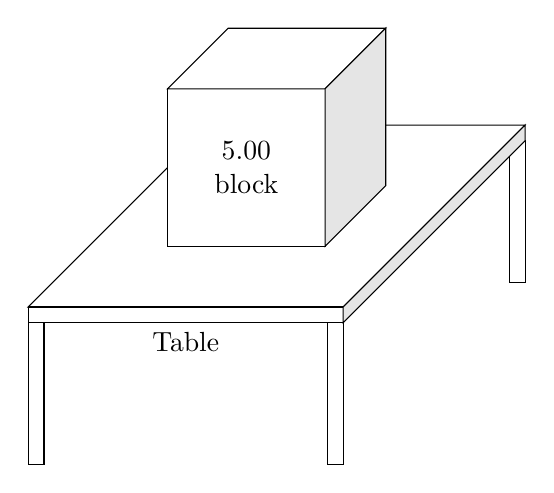
\begin{tikzpicture}
        %% legs
        \draw (-2,-0.2,-4) rectangle (-1.8,-2,-4);
        \draw (+2,-0.2,-4) rectangle (+1.8,-2,-4);
        \draw (-2,-0.2,+2) rectangle (-1.8,-2,+2);
        \draw (+2,-0.2,+2) rectangle (+1.8,-2,+2);
        %% table
        \draw[fill=white] (-2,0,2) -- (-2,0,-4) -- (2,0,-4) -- (2,0,2) -- cycle;
        \draw (-2,0,2) -- (-2,-0.2,2) -- (2,-0.2,2) -- (2,0,2) -- cycle;
        \draw[fill=white!90!black] (2,0,2) -- (2,0,-4) -- (2,-0.2,-4) -- (2,-0.2,2) -- cycle;
        \node[anchor=north] at (0,-0.2,2) {Table};
        %% 5 kg block
        \draw[fill=white] (-1,0,0) -- (1,0,0) -- (1,2,0) -- (-1,2,0) -- cycle;
        \node[anchor=center,text centered,text width=3em] at (0,1,0) {\SI{5.00}{\kilo\gram} block};
        \draw[fill=white] (-1,2,0) -- (-1,2,-2) -- (1,2,-2) -- (1,2,0)  -- cycle;
        \draw[fill=white!90!black] (1,0,0) -- (1,0,-2) -- (1,2,-2) -- (1,2,0) -- cycle; 
    \end{tikzpicture}
    \end{center}
    Which diagram best represents the force exerted on the block by the table?
    \begin{multicols}{2}
    \begin{choices}\small
        \AMCboxDimensions{down=-1.2cm}
        \correctchoice{
            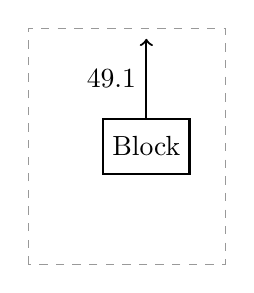
\begin{tikzpicture}
                \draw[dashed,white!60!black] (-1.5,-1.5) rectangle (1,1.5);
                \node[draw,thick,rectangle,anchor=center,minimum size=2em] (B) at (0,0) {Block};
                \draw[thick,->] (B.north) -- ++(90:1)
                    node[pos=0.5,anchor=east] {\SI{49.1}{\newton}};
            \end{tikzpicture}
        }
        \wrongchoice{
            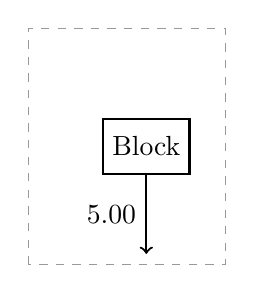
\begin{tikzpicture}
                \draw[dashed,white!60!black] (-1.5,-1.5) rectangle (1,1.5);
                \node[draw,thick,rectangle,anchor=center,minimum size=2em] (B) at (0,0) {Block};
                \draw[thick,->] (B.south) -- ++(270:1)
                    node[pos=0.5,anchor=east] {\SI{5.00}{\newton}};
            \end{tikzpicture}
        }
        \wrongchoice{
            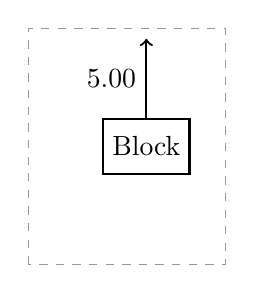
\begin{tikzpicture}
                \draw[dashed,white!60!black] (-1.5,-1.5) rectangle (1,1.5);
                \node[draw,thick,rectangle,anchor=center,minimum size=2em] (B) at (0,0) {Block};
                \draw[thick,->] (B.north) -- ++(90:1)
                    node[pos=0.5,anchor=east] {\SI{5.00}{\kilo\gram}};
            \end{tikzpicture}
        }
        \wrongchoice{
            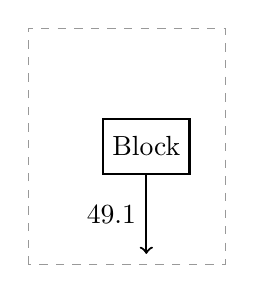
\begin{tikzpicture}
                \draw[dashed,white!60!black] (-1.5,-1.5) rectangle (1,1.5);
                \node[draw,thick,rectangle,anchor=center,minimum size=2em] (B) at (0,0) {Block};
                \draw[thick,->] (B.south) -- ++(270:1)
                    node[pos=0.5,anchor=east] {\SI{49.1}{\kilo\gram}};
            \end{tikzpicture}
        }
    \end{choices}
    \end{multicols}
\end{question}
}

\element{nysed}{
\begin{question}{June2005-Q45}
    The diagram below represents a block at rest on an incline.
    \begin{center}
    \begin{tikzpicture}[scale=1.33]
        \node[draw,minimum size=1cm,rotate=30,anchor=south] at (30:3) {Block};
        \draw[thick] (0,0) -- (30:4) -- ++(270:{4*sin(30)});
        %% Floor
        \draw[thick] (-1,0) -- (4,0) node[pos=0.5,anchor=north,yshift=-1em] {Horizontal};
        \node[anchor=north,pattern=north east lines,minimum width=6.65cm] at (1.5,0) {};
    \end{tikzpicture}
    \end{center}
    Which diagram best represents the forces acting on the block?
    ($F_f =\text{frictional force}$, $F_N=\text{normal force}$, and $F_w=\text{weight}$.)
    \begin{multicols}{2}
    \begin{choices}
        \AMCboxDimensions{down=-1.25cm}
        \correctchoice{
            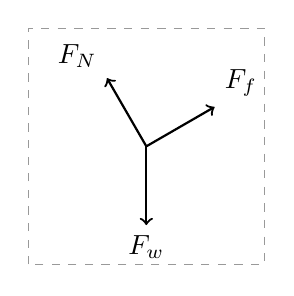
\begin{tikzpicture}
                \draw[dashed,white!60!black] (-1.5,-1.5) rectangle (1.5,1.5);
                \draw[thick,->] (0,0) -- (120:1) node[anchor=south east] {$F_N$};
                \draw[thick,->] (0,0) -- (30:1)  node[anchor=south west] {$F_f$};
                \draw[thick,->] (0,0) -- (270:1) node[anchor=north] {$F_w$};
            \end{tikzpicture}
        }
        \wrongchoice{
            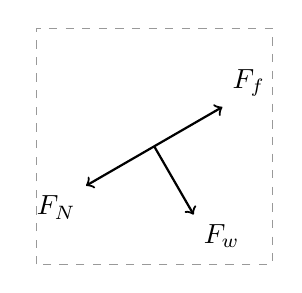
\begin{tikzpicture}
                \draw[dashed,white!60!black] (-1.5,-1.5) rectangle (1.5,1.5);
                \draw[thick,->] (0,0) -- (210:1) node[anchor=north east] {$F_N$};
                \draw[thick,->] (0,0) -- (30:1)  node[anchor=south west] {$F_f$};
                \draw[thick,->] (0,0) -- (300:1) node[anchor=north west] {$F_w$};
            \end{tikzpicture}
        }
        \wrongchoice{
            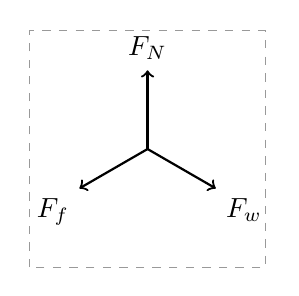
\begin{tikzpicture}
                \draw[dashed,white!60!black] (-1.5,-1.5) rectangle (1.5,1.5);
                \draw[thick,->] (0,0) -- (90:1)  node[anchor=south] {$F_N$};
                \draw[thick,->] (0,0) -- (210:1) node[anchor=north east] {$F_f$};
                \draw[thick,->] (0,0) -- (330:1) node[anchor=north west] {$F_w$};
            \end{tikzpicture}
        }
        \wrongchoice{
            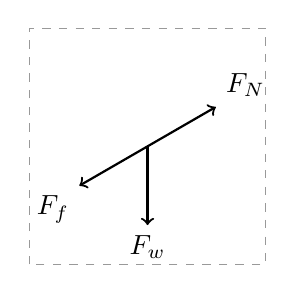
\begin{tikzpicture}
                \draw[dashed,white!60!black] (-1.5,-1.5) rectangle (1.5,1.5);
                \draw[thick,->] (0,0) -- (30:1)  node[anchor=south west] {$F_N$};
                \draw[thick,->] (0,0) -- (210:1) node[anchor=north east] {$F_f$};
                \draw[thick,->] (0,0) -- (270:1) node[anchor=north] {$F_w$};
            \end{tikzpicture}
        }
    \end{choices}
    \end{multicols}
\end{question}
}


%% Section Jan2005
%%--------------------
\element{nysed}{
\begin{question}{Jan2005-Q09}
    The diagram below shows a sled and rider sliding down a snow covered hill that makes an angle of \ang{30} with the horizontal.
    \begin{center}
    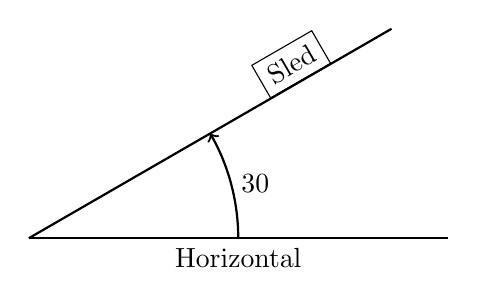
\begin{tikzpicture}[scale=1.33]
        \draw[thick] (0,0) -- (4,0) node[anchor=north,pos=0.5] {Horizontal};
        \node[draw,minimum size=1em,rotate=30,anchor=south] at (30:3) {Sled};
        \draw[thick] (0,0) -- (30:4);
        \draw[thick,->] (0:2) arc(0:30:2) node[pos=0.5,anchor=west] {\ang{30}};
    \end{tikzpicture}
    \end{center}
    Which vector best represents the direction of the normal force, $F_N$, exerted by the hill on the sled?
    \begin{multicols}{2}
    \begin{choices}\small
        \AMCboxDimensions{down=-1.40cm}
        \correctchoice{
            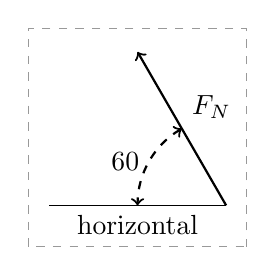
\begin{tikzpicture}[scale=0.75]
                \draw[dashed,white!60!black] (1em,-2em) rectangle (-3cm-1em,3cm);
                \draw (0,0) -- (-3,0)
                    node[pos=0.5,anchor=north] {horizontal};
                \draw[thick,->] (0,0) -- ++(120:3)
                    node[pos=0.5,anchor=south west] {$F_N$};
                \draw[dashed,thick,<->] (120:1.5) arc (120:180:1.5)
                    node[pos=0.5,anchor=east] {\ang{60}};
            \end{tikzpicture}
        }
        \wrongchoice{
            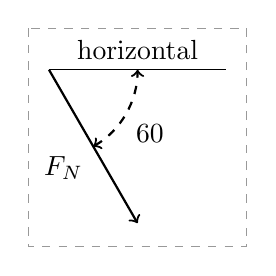
\begin{tikzpicture}[scale=0.75]
                \draw[dashed,white!60!black] (-1em,2em) rectangle (3cm+1em,-3cm);
                \draw (0,0) -- (3,0)
                    node[pos=0.5,anchor=south] {horizontal};
                \draw[thick,->] (0,0) -- ++(300:3)
                    node[pos=0.5,anchor=north east] {$F_N$};
                \draw[dashed,thick,<->] (300:1.5) arc (300:360:1.5)
                    node[pos=0.5,anchor=north west] {\ang{60}};
            \end{tikzpicture}
        }
        \wrongchoice{
            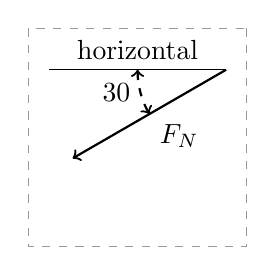
\begin{tikzpicture}[scale=0.75]
                \draw[dashed,white!60!black] (1em,+2em) rectangle (-3cm-1em,-3cm);
                \draw (0,0) -- (-3,0)
                    node[pos=0.5,anchor=south] {horizontal};
                \draw[thick,->] (0,0) -- ++(210:3)
                    node[pos=0.5,anchor=north west] {$F_N$};
                \draw[dashed,thick,<->] (180:1.5) arc (180:210:1.5)
                    node[pos=0.5,anchor=east] {\ang{30}};
            \end{tikzpicture}
        }
        \wrongchoice{
            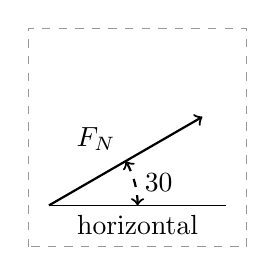
\begin{tikzpicture}[scale=0.75]
                \draw[dashed,white!60!black] (-1em,-2em) rectangle (3cm+1em,3cm);
                \draw (0,0) -- (3,0)
                    node[pos=0.5,anchor=north] {horizontal};
                \draw[thick,->] (0,0) -- ++(30:3)
                    node[pos=0.5,anchor=south east] {$F_N$};
                \draw[dashed,thick,<->] (0:1.5) arc (0:30:1.5)
                    node[pos=0.5,anchor=west] {\ang{30}};
            \end{tikzpicture}
        }
    \end{choices}
    \end{multicols}
\end{question}
}


%% Section June2004
%%--------------------
\element{nysed}{
\begin{question}{June2004-Q08}
    The force required to start an object sliding across a uniform horizontal surface is larger than the force required to keep the object sliding at a constant velocity.
    The magnitudes of the required forces are different in these situations because the force of kinetic friction:
    \begin{choices}
      \correctchoice{is less than the force of static friction}
        \wrongchoice{is greater than the force of static friction}
        \wrongchoice{increases as the speed of the object relative to the surface increases}
        \wrongchoice{decreases as the speed of the object relative to the surface increases}
    \end{choices}
\end{question}
}


%% Section Jan2004
%%--------------------
\element{nysed}{
\begin{question}{Jan2004-Q10}
    A box is pushed toward the right across a classroom floor.
    The force of friction on the box is directed toward the:
    \begin{multicols}{2}
    \begin{choices}
      \correctchoice{left}
        \wrongchoice{right}
        \wrongchoice{ceiling}
        \wrongchoice{floor}
    \end{choices}
    \end{multicols}
\end{question}
}


%% Section June2003
%%--------------------
\element{nysed}{
\begin{question}{June2003-Q47}
    Three forces act on a box on an inclined plane as shown in the diagram below.
    Vectors are not drawn to scale.
    \begin{center}
    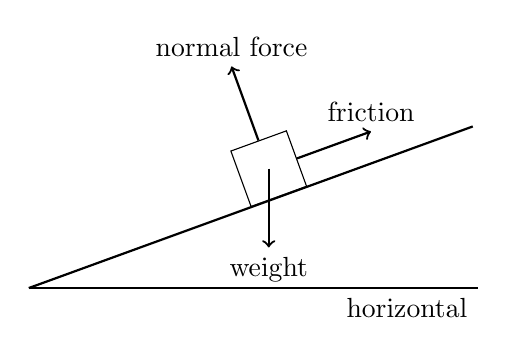
\begin{tikzpicture}
        %% Ramp and floor
        \draw[thick] (0,0) -- (20:6);
        \draw[thick] (0:0) -- (0:5.7)
            node[pos=1.0,anchor=north east] {horizontal};
        %% Block
        \node[draw,rectangle,minimum size=0.75cm,rotate=20,anchor=south west]
            (B) at (20:3) {};
        %% Three Forces
        \draw[thick,->] (B.north) -- ++(110:1)
            node[pos=1.0,anchor=south] {normal force};
        \draw[thick,->] (B.center) -- ++(270:1)
            node[pos=1.0,anchor=north] {weight};
        \draw[thick,->] (B.east) -- ++(20:1)
            node[pos=1.0,anchor=south] {friction};
    \end{tikzpicture}
    \end{center}
    If the box is at rest,
        the net force acting on it is equal to:
    \begin{multicols}{2}
    \begin{choices}
      \correctchoice{zero}
        \wrongchoice{the weight}
        \wrongchoice{friction}
        \wrongchoice{the normal force}
    \end{choices}
    \end{multicols}
\end{question}
}


%% Section Jan2003
%%--------------------
\element{nysed}{
\begin{question}{Jan2003-Q11}
    The diagram below shows a block sliding down a plane inclined at angle $\theta$ with the horizontal.
    \begin{center}
    \begin{tikzpicture}
        %% Plane with Box
        \node[draw,minimum size=1cm,rotate=30,anchor=south] at (30:3) {};
        \draw[thick] (0,0) -- (30:4);
        \draw[dashed,thick,<->] (0:2) arc(0:30:2) node[pos=0.5,anchor=west] {$\theta$};
        %% Floor
        \draw[thick] (0,0) -- (4,0);
        \node[pattern=north east lines,anchor=north,minimum width=4cm] at (2,0) {};
    \end{tikzpicture}
    \end{center}
    As angle $\theta$ is increased,
        the coefficient of kinetic friction between the bottom surface of the block and the surface of the incline will:
    \begin{choices}
      \correctchoice{decrease}
        \wrongchoice{increase}
        \wrongchoice{remain the same}
    \end{choices}
\end{question}
}


%% Section Aug2002
%%--------------------
\element{nysed}{
\begin{question}{Aug2002-Q05}
    In the diagram below, a box is at rest on an inclined plane.
    \begin{center}
    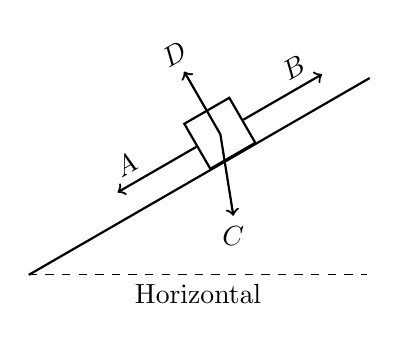
\begin{tikzpicture}
        %% Ramp
        \draw[thick] (0,0) -- (30:5cm);
        \draw[dashed] (0,0) -- (4.3,0)
            node[pos=0.5,anchor=north] {Horizontal};
        %% Block
        \node[thick,draw,rectangle,minimum size=0.66cm,rotate=30,anchor=south] 
            (B) at (30:3cm) {};
        \draw[thick,->] (B) -- ++ (210:1.5cm)
            node[anchor=south west,rotate=30] {$A$};
        \draw[thick,->] (B) -- ++ (30:1.5cm)
            node[anchor=south east,rotate=30] {$B$};
        \draw[thick,->] (30:3cm) +(120:0.33cm) -- ++ (270:0.75cm)
            node[anchor=north] {$C$};
        \draw[thick,->] (30:3cm) +(120:0.33cm) -- ++ (120:1.25cm)
            node[anchor=south,rotate=30] {$D$};
    \end{tikzpicture}
    \end{center}
    Which vector best represents the direction of the normal force acting on the box?
    \begin{multicols}{4}
    \begin{choices}[o]
        \wrongchoice{$A$}
        \wrongchoice{$B$}
      \correctchoice{$C$}
        \wrongchoice{$D$}
    \end{choices}
    \end{multicols}
\end{question}
}

\element{nysed}{
\begin{question}{Aug2002-Q08}
    A block weighing \SI{15}{\newton} is pulled to the top of an incline that is \SI{0.20}{\meter} above the ground, as shown below.
    \begin{center}
    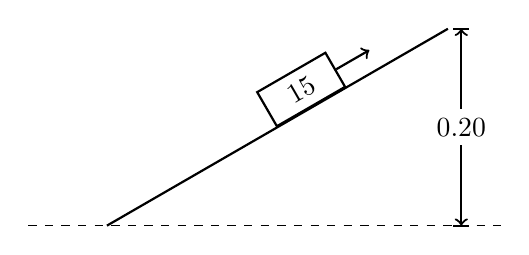
\begin{tikzpicture}
        %% Ramp 5cm wide
        \draw[thick] (0,0) -- (30:5cm);
        \draw[dashed] (-1,0) -- (5,0);
        \draw[thick] (4.4,0.0) -- (4.6,0.0);
        \draw[thick] (4.4,2.5) -- (4.6,2.5);
        \draw[thick,<->] (4.5,0) -- (4.5,2.5)
            node[fill=white,pos=0.5,anchor=center] {\SI{0.20}{\meter}};
        %% Block
        \node[thick,draw,rectangle,minimum width=1cm,minimum height=0.5cm,rotate=30,anchor=south] 
            (B) at (30:3cm) {\SI{15}{\newton}};
        \draw[thick,->] (B) -- ++ (30:1cm);
    \end{tikzpicture}
    \end{center}
    If \SI{4.0}{\joule} of work are needed to pull the block the full length of the incline,
        how much work is done against friction?
    \begin{multicols}{2}
    \begin{choices}
      \correctchoice{\SI{1.0}{\joule}}
        \wrongchoice{\SI{0.0}{\joule}}
        \wrongchoice{\SI{3.0}{\joule}}
        \wrongchoice{\SI{7.0}{\joule}}
    \end{choices}
    \end{multicols}
\end{question}
}

\element{nysed}{
\begin{question}{Aug2002-Q37}
    The diagram below shows a \SI{10.0}{\kilo\gram} mass held at rest on a frictionless \ang{30.0} incline by force $F$.
    \begin{center}
    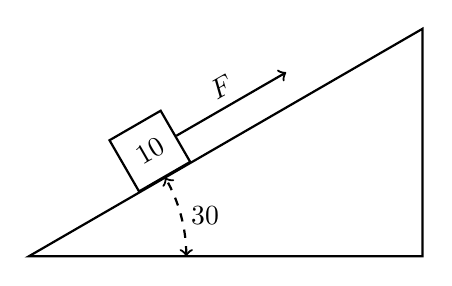
\begin{tikzpicture}
        %% Ramp
        \draw[thick] (0,0) -- (5.00,2.89) -- (5.00,0.0) -- cycle;
        \draw[thick,dashed,<->] (0:2.0) arc (0:30:2.0)
            node[pos=0.5,anchor=west] {\ang{30}};
        %% Block
        \node[thick,draw,rectangle,minimum size=0.75cm,rotate=30,anchor=south] 
            (B) at (30:2cm) {\SI{10}{\kilo\gram}};
        \draw[thick,->] (B) -- ++ (30:2cm)
            node[pos=0.5,anchor=south,rotate=30] {$F$};
    \end{tikzpicture}
    \end{center}
    What is the approximate magnitude of force $F$?
    \begin{multicols}{2}
    \begin{choices}
        \wrongchoice{\SI{9.81}{\newton}}
      \correctchoice{\SI{49.1}{\newton}}
        \wrongchoice{\SI{85.0}{\newton}}
        \wrongchoice{\SI{98.1}{\newton}}
    \end{choices}
    \end{multicols}
\end{question}
}


%% Section June2002
%%--------------------
\element{nysed}{
\begin{question}{June2002-Q02}
    The diagram below shows a granite block being slide at constant speed across a horizontal concrete floor by a force parallel to the floor.
    \begin{center}
        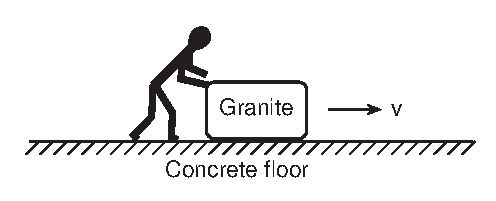
\includegraphics[keepaspectratio,scale=0.9]{June2002-Q02}
    \end{center}
    Which pair of quantities could be used to determine the coefficient of friction for the granite on the concrete?
    \begin{choices}
        \wrongchoice{mass and speed of the block}
        \wrongchoice{mass and normal force on the block}
        \wrongchoice{frictional force and speed of the block}
      \correctchoice{frictional force and normal force on the block}
    \end{choices}
\end{question}
}

%% Section Jan2002
%%--------------------
\element{nysed}{
\begin{question}{Jan2002-Q12}
    The table below lists the coefficients of kinetic friction for four materials sliding over steel.
    \begin{center}
    \begin{tabu}{X[c]X[c]}
        \toprule
        Material & Coefficient of Kinetic Friction \\
        \midrule
        aluminum    & 0.47 \\
        brass       & 0.44 \\
        copper      & 0.36 \\
        steel       & 0.57 \\
        \bottomrule
    \end{tabu}
    \end{center}
    A \SI{10}{\kilo\gram} block of each of these materials is pulled horizontally across a steel floor at constant velocity.
    Which block requires the \emph{smallest} applied force to keep it moving at constant velocity?
    \begin{multicols}{2}
    \begin{choices}
        \wrongchoice{aluminum}
        \wrongchoice{brass}
      \correctchoice{copper}
        \wrongchoice{steel}
    \end{choices}
    \end{multicols}
\end{question}
}


%% Section June2001
%%--------------------
\element{nysed}{
\begin{question}{June2001-Q10}
    A \SI{50}{\newton} horizontal force is needed to keep an object weighing \SI{500}{\newton} moving at a constant velocity of \SI{2.0}{\meter\per\second} across a horizontal surface.
    The magnitude of the frictional force acting on the object is:
    \begin{multicols}{2}
    \begin{choices}
      \correctchoice{\SI{500}{\newton}}
        \wrongchoice{\SI{450}{\newton}}
        \wrongchoice{\SI{50}{\newton}}
        \wrongchoice{\SI{0}{\newton}}
    \end{choices}
    \end{multicols}
\end{question}
}

\element{nysed}{
\begin{question}{June2001-Q11}
    The diagram below represents a block sliding down an incline.
    \begin{center}
    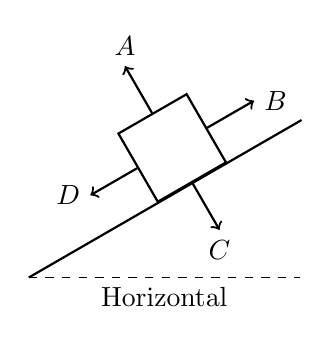
\begin{tikzpicture}[scale=0.8]
        %% Ramp
        \draw[thick] (0,0) -- (30:5cm);
        \draw[dashed] (0,0) -- (4.3,0)
            node[pos=0.5,anchor=north] {Horizontal};
        %% Block
        \node[thick,draw,rectangle,minimum size=1.00cm,rotate=30,anchor=south] (B) at (30:3cm) {};
        %% Vectors
        \draw[thick,->] (B) --++ (120:1.5cm)
            node[anchor=south] {$A$};
        \draw[thick,->] (B) --++ (30:1.5cm)
            node[anchor=west] {$B$};
        \draw[thick,->] (B) --++ (-60:1.5cm)
            node[anchor=north] {$C$};
        \draw[thick,->] (B) --++ (210:1.5cm)
            node[anchor=east] {$D$};
    \end{tikzpicture}
    \end{center}
    Which vector best represents the frictional force acting on the block?
    \begin{multicols}{4}
    \begin{choices}[o]
        \wrongchoice{$A$}
      \correctchoice{$B$}
        \wrongchoice{$C$}
        \wrongchoice{$D$}
    \end{choices}
    \end{multicols}
\end{question}
}

\element{nysed}{
\begin{question}{June2001-Q12}
    A different force is applied to each of four \SI{1}{\kilo\gram} blocks to slide them across a uniform steel surface at constant speed as shown below.
    In which diagram is the coefficient of friction between the block and steel \emph{smallest}?
    \begin{multicols}{2}
    \begin{choices}
        \AMCboxDimensions{down=-0.50cm}
        \correctchoice{
            \begin{tikzpicture}[font=\footnotesize,xscale=0.66]
                %% Force
                \draw[thick,->] (-2,0.5) -- (0,0.5)
                    node[pos=1.0,anchor=south east] {$F=\SI{2}{\newton}$};
                %% Block
                \draw[thick] (0,0) rectangle (2,1);
                \node[anchor=center,text width=3em,text centered]
                    at (1,0.5) {\SI{1}{\kilo\gram} Block};
                %% Floor
                \draw[thick] (-2,0) -- (2.5,0);
                \node[anchor=north,minimum width=3cm,pattern=north east lines] at (0.25,0) {};
                \node[anchor=north] at (0,-0.2) {Steel};
            \end{tikzpicture}
        }
        \wrongchoice{
            \begin{tikzpicture}[font=\footnotesize,xscale=0.66]
                %% Force
                \draw[thick,->] (-2,0.5) -- (0,0.5)
                    node[pos=1.0,anchor=south east] {$F=\SI{5}{\newton}$};
                %% Block
                \draw[thick] (0,0) rectangle (2,1);
                \draw[thick] (0,0) rectangle (2,1);
                \node[anchor=center,text width=3em,text centered]
                    at (1,0.5) {\SI{1}{\kilo\gram} Block};
                %% Floor
                \draw[thick] (-2,0) -- (2.5,0);
                \node[anchor=north,minimum width=3cm,pattern=north east lines] at (0.25,0) {};
                \node[anchor=north] at (0,-0.2) {Steel};
            \end{tikzpicture}
        }
        \wrongchoice{
            \begin{tikzpicture}[font=\footnotesize,xscale=0.66]
                %% Force
                \draw[thick,->] (-2,0.5) -- (0,0.5)
                    node[pos=1.0,anchor=south east] {$F=\SI{3}{\newton}$};
                %% Block
                \draw[thick] (0,0) rectangle (2,1);
                \node[anchor=center,text width=3em,text centered]
                    at (1,0.5) {\SI{1}{\kilo\gram} Block};
                %% Floor
                \draw[thick] (-2,0) -- (2.5,0);
                \node[anchor=north,minimum width=3cm,pattern=north east lines] at (0.25,0) {};
                \node[anchor=north] at (0,-0.2) {Steel};
            \end{tikzpicture}
        }
        \wrongchoice{
            \begin{tikzpicture}[font=\footnotesize,xscale=0.66]
                %% Force
                \draw[thick,->] (-2,0.5) -- (0,0.5)
                    node[pos=1.0,anchor=south east] {$F=\SI{4}{\newton}$};
                %% Block
                \draw[thick] (0,0) rectangle (2,1);
                \node[anchor=center,text width=3em,text centered]
                    at (1,0.5) {\SI{1}{\kilo\gram} Block};
                %% Floor
                \draw[thick] (-2,0) -- (2.5,0);
                \node[anchor=north,minimum width=3cm,pattern=north east lines] at (0.25,0) {};
                \node[anchor=north] at (0,-0.2) {Steel};
            \end{tikzpicture}
        }
    \end{choices}
    \end{multicols}
\end{question}
}


%% Section Jan2001
%%--------------------
\element{nysed}{
\begin{question}{Jan2001-Q15}
    A wooden block is at rest on a horizontal steel surface.
    If a \SI{10}{\newton} force applied parallel to the surface is required to set the block in motion,
        how much force is required to keep the block moving at constant velocity?
    \begin{choices}
        \wrongchoice{less than \SI{10}{\newton}}
        \wrongchoice{greater than \SI{10}{\newton}}
      \correctchoice{\SI{10}{\newton}}
    \end{choices}
\end{question}
}


%% Section June2000
%%--------------------
\element{nysed}{
\begin{question}{June2000-Q04}
    A cart moving across a level surface accelerates uniformly at \SI{1.0}{\meter\per\second\squared}.
    What additional information is required to determine the distance traveled by the cart during this \SI{2.0}{\second} interval?
    \begin{choices}
        \wrongchoice{coefficient of friction between the cart and the surface}
        \wrongchoice{mass of the cart}
        \wrongchoice{net force acting on the cart}
      \correctchoice{initial velocity of the cart}
    \end{choices}
\end{question}
}

\element{nysed}{
\begin{question}{June2000-Q14}
    Sand is often placed on an icy road because the sand:
    \begin{choices}
        \wrongchoice{decreases the coefficient of friction between the tire and the road}
      \correctchoice{increases the coefficient of friction between the tire and the road}
        \wrongchoice{decreases the gravitational force on the car}
        \wrongchoice{increases the normal force of a car on the road}
    \end{choices}
\end{question}
}



%% Section June1999
%%--------------------
\element{nysed}{
\begin{question}{June1999-Q08}
    If a \SI{30}{\newton} force is required to accelerate a \SI{2}{\kilo\gram} object at \SI{10}{\meter\per\second},
        over a level floor, then the magnitude of the frictional force acting on the object is:
    \begin{multicols}{2}
    \begin{choices}
        \wrongchoice{\SI{0}{\newton}}
      \correctchoice{\SI{10}{\newton}}
        \wrongchoice{\SI{20}{\newton}}
        \wrongchoice{\SI{30}{\newton}}
    \end{choices}
    \end{multicols}
\end{question}
}

\element{nysed}{
\begin{question}{June1999-Q09}
    The diagram below shows a stuent applying a \SI{10}{\newton} force to slide a piece of wood at constant speed across a horizontal surface.
    After the wood is cut in half, one piece is placed on top of the other, as shown.
    \begin{center}
    \begin{tikzpicture}
        %% NOTE: TODO: draw tikz
        %% 3d cube??
        %% rectangle object and make 3d??
        \begin{scope}[xshift=-2cm]
        \end{scope}
    \end{tikzpicture}
    \end{center}
    What is the magnitude of the force, $F$,
        required to slide the stacked wood at constant speed across the surface?
    \begin{multicols}{2}
    \begin{choices}
        \wrongchoice{\SI{40}{\newton}}
        \wrongchoice{\SI{20}{\newton}}
      \correctchoice{\SI{10}{\newton}}
        \wrongchoice{\SI{5.0}{\newton}}
    \end{choices}
    \end{multicols}
\end{question}
}

\element{nysed}{
\begin{question}{June1999-Q10}
    In the diagram below, a block rests on a ramp,
        making an angle $\theta$ with the horizontal.
    \begin{center}
    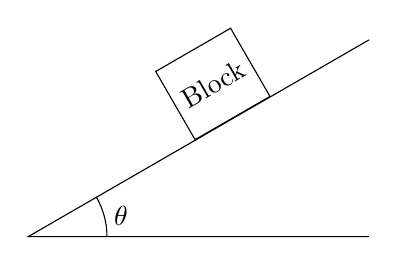
\begin{tikzpicture}
        %% ramp
        \draw ({5*cos(30)},0) -- (0,0) -- (30:5);
        \draw (1,0) arc (0:30:1) node[pos=0.5,anchor=west] {$\theta$};
        %% block
        \node[draw,anchor=south,rotate=30,minimum size=1cm] at (30:3) {Block};
    \end{tikzpicture}
    \end{center}
    If angle $\theta$ is increased, what will occur?
    \begin{choices}
        \wrongchoice{The block's mass will decrease.}
        \wrongchoice{The block's weight will increase.}
        \wrongchoice{The block's component of weight parallel to the ramp will decrease.}
      \correctchoice{The block's component of weight parallel to the ramp will increase.}
    \end{choices}
\end{question}
}


%% Section June1998
%%--------------------
\element{nysed}{
\begin{question}{June1998-Q06}
    A \SI{1.0}{\kilo\gram} block is placed on each of four frictionless planes inclined at different angles.
    On which inclined plane will the acceleration of the block be greatest?
    \begin{multicols}{2}
    \begin{choices} \small
        \AMCboxDimensions{down=-0.5cm}
        \wrongchoice{
            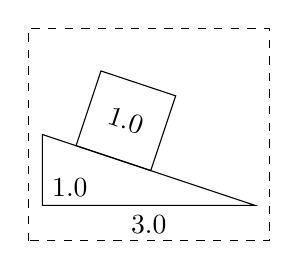
\begin{tikzpicture}[scale=0.9]
                \draw[dashed] (-0.2,-0.5) rectangle (3.2,2.5);
                \draw (0,0) -- (0,1) -- (3,0) -- cycle;
                \node[anchor=north] at (1.5,0) {\SI{3.0}{\meter}};
                \node[anchor=west] at (0,0.25) {\SI{1.0}{\meter}};
                \node[draw,anchor=south,rotate=-18.43,minimum size=1cm] at (1,0.66) {\SI{1.0}{\kilo\gram}};
            \end{tikzpicture}
        }
        \wrongchoice{
            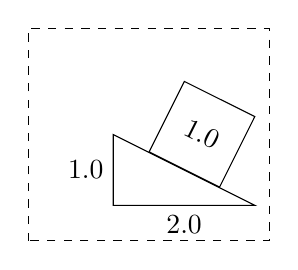
\begin{tikzpicture}[scale=0.9]
                \draw[dashed] (-1.2,-0.5) rectangle (2.2,2.5);
                \draw (0,0) -- (0,1) -- (2,0) -- cycle;
                \node[anchor=north] at (1,0) {\SI{2.0}{\meter}};
                \node[anchor=east] at (0,0.5) {\SI{1.0}{\meter}};
                \node[draw,anchor=south,rotate=-26.56,minimum size=1cm] at (1,0.5) {\SI{1.0}{\kilo\gram}};
            \end{tikzpicture}
        }
        \wrongchoice{
            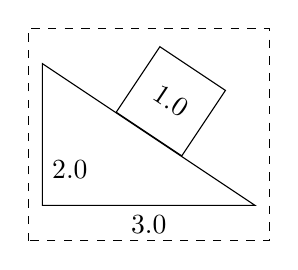
\begin{tikzpicture}[scale=0.9]
                \draw[dashed] (-0.2,-0.5) rectangle (3.2,2.5);
                \draw (0,0) -- (0,2) -- (3,0) -- cycle;
                \node[anchor=north] at (1.5,0) {\SI{3.0}{\meter}};
                \node[anchor=west] at (0,0.5) {\SI{2.0}{\meter}};
                \node[draw,anchor=south,rotate=-33.69,minimum size=1cm] at (1.5,1) {\SI{1.0}{\kilo\gram}};
            \end{tikzpicture}
        }
        \correctchoice{
            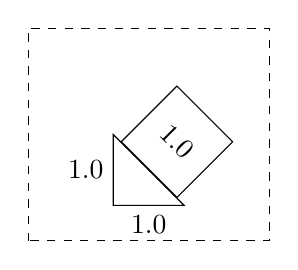
\begin{tikzpicture}[scale=0.9]
                \draw[dashed] (-1.2,-0.5) rectangle (2.2,2.5);
                \draw (0,0) -- (0,1) -- (1,0) -- cycle;
                \node[anchor=north] at (0.5,0) {\SI{1.0}{\meter}};
                \node[anchor=east] at (0,0.5) {\SI{1.0}{\meter}};
                \node[draw,anchor=south,rotate=-45,minimum size=1cm] at (0.5,0.5) {\SI{1.0}{\kilo\gram}};
            \end{tikzpicture}
        }
    \end{choices}
    \end{multicols}
\end{question}
}

\element{nysed}{
\begin{question}{June1998-Q12}
    A book weighing \SI{20}{\newton} slides at constant velocity down a ramp inclined \ang{30} to the horizontal as shown in the diagram below.
    \begin{center}
    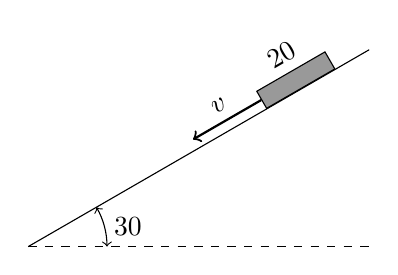
\begin{tikzpicture}
        %% incline
        \draw (0,0) -- (30:5);
        \draw[dashed] (0,0) -- ({5*cos(30)},0);
        \draw[<->] (1,0) arc (0:30:1) node[pos=0.5,anchor=west] {\ang{30}};
        %% book
        \node[draw,fill=white!60!black,minimum width=1cm,minimum height=0.25cm,anchor=south,rotate=30] (B) at (30:4) {};
        \node[anchor=south,rotate=30] at (B.north) {\SI{20}{\newton}};
        \draw[thick,->] (B.west) -- ++(210:1) node[pos=0.5,anchor=south,rotate=30] {$v$};
    \end{tikzpicture}
    \end{center}
    What is the force of friction between the book and the ramp?
    \begin{choices}
        \wrongchoice{\SI{10}{\newton} up the ramp}
        \wrongchoice{\SI{17}{\newton} up the ramp}
        \wrongchoice{\SI{10}{\newton} down the ramp}
      \correctchoice{\SI{17}{\newton} down the ramp}
    \end{choices}
\end{question}
}


%% Section June1997
%%--------------------
\element{nysed}{
\begin{question}{June1997-Q13}
    In the diagram below, surface $B$ of the wooden block has the same texture of surface $A$,
        but twice the area of surface $A$.
    \begin{center}
    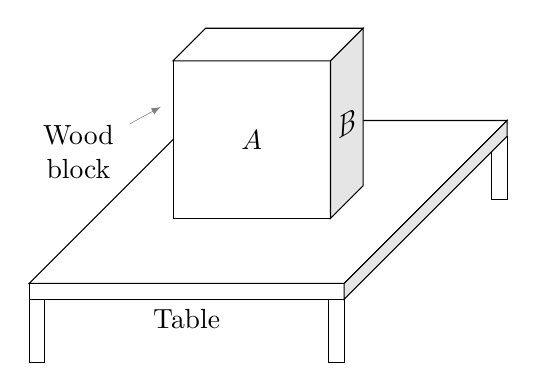
\begin{tikzpicture}
        %\pgfsetxvec{\pgfpoint{.866cm}{.5cm}}
        %\pgfsetyvec{\pgfpoint{.866cm}{-.5cm}}
        \pgfsetzvec{\pgfpoint{-0.414cm}{-0.414cm}}
        %% legs
        \draw (-2,-0.2,-3) rectangle (-1.8,-1,-3);
        \draw (+2,-0.2,-3) rectangle (+1.8,-1,-3);
        \draw (-2,-0.2,+2) rectangle (-1.8,-1,+2);
        \draw (+2,-0.2,+2) rectangle (+1.8,-1,+2);
        %% table
        \draw[fill=white] (-2,0,2) -- (-2,0,-3) -- (2,0,-3) -- (2,0,2) -- cycle;
        \draw[fill=white] (-2,0,2) -- (-2,-0.2,2) -- (2,-0.2,2) -- (2,0,2) -- cycle;
        \draw[fill=white!90!black] (2,0,2) -- (2,0,-3) -- (2,-0.2,-3) -- (2,-0.2,2) -- cycle;
        \node[anchor=north] at (0,-0.2,2) {Table};
        %% 5 kg block
        \draw[fill=white] (-1,0,0) -- (1,0,0) -- (1,2,0) -- (-1,2,0) -- cycle;
        \node[anchor=center] at (0,1,0) {$A$};
        \draw[fill=white] (-1,2,0) -- (-1,2,-1) -- (1,2,-1) -- (1,2,0)  -- cycle;
        \draw[fill=white!90!black] (1,0,0) -- (1,0,-1) -- (1,2,-1) -- (1,2,0) -- cycle; 
        \node[anchor=center,rotate=30,xslant=0.414] at (1,1,-0.5) {$B$};
        \node[pin={[text centered,text width=3em,pin edge={latex-,shorten <=1pt}]200:Wood block}] at (-1,1.5,0) {};
    \end{tikzpicture}
    \end{center}
    If force $F$ is required to slide the block at constant speed across the table on surface $A$,
        approximately what force is required to slide the block at constant speed across the table on surface $B$?
    \begin{multicols}{4}
    \begin{choices}
      \correctchoice{$F$}
        \wrongchoice{$2F$}
        \wrongchoice{$\dfrac{F}{2}$}
        \wrongchoice{$4F$}
    \end{choices}
    \end{multicols}
\end{question}
}

\element{nysed}{
\begin{question}{June1997-Q57}
    A soccer ball travels the path shown in the diagram below.
    \begin{center}
    \begin{tikzpicture}
        %% Ground
        \node[anchor=north,fill,pattern=north east lines,minimum width=8cm, minimum height=0.05cm] at (3,0) {};
        \draw (-1,0) -- (7,0);
        %% path
        \draw[dashed] (0,0) parabola bend (3,2) (6,0);
        %% label
        \draw[very thick,-latex] (0.75,0.875) -- ++(45:1);
        \draw[very thick,fill=white] (0.75,0.875) circle (2.5pt) node[anchor=south east] {$P$};
    \end{tikzpicture}
    \end{center}
    Which vector best represents the direction of the force of air friction on the ball at point $P$?
    \begin{multicols}{2}
    \begin{choices}
        \AMCboxDimensions{down=-0.8cm}
        \wrongchoice{
            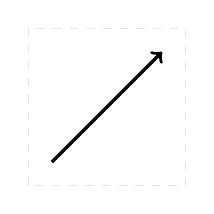
\begin{tikzpicture}[scale=2]
                \draw[dashed,white!90!black] (0,0) rectangle (1,1);
                \draw[very thick,->] (0.15,0.15) -- (0.85,0.85);
            \end{tikzpicture}
        }
        \correctchoice{
            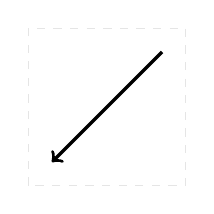
\begin{tikzpicture}[scale=2]
                \draw[dashed,white!90!black] (0,0) rectangle (1,1);
                \draw[very thick,->] (0.85,0.85) -- (0.15,0.15);
            \end{tikzpicture}
        }
        \wrongchoice{
            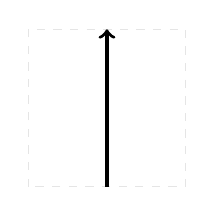
\begin{tikzpicture}[scale=2]
                \draw[dashed,white!90!black] (0,0) rectangle (1,1);
                \draw[very thick,->] (0.5,0) -- (0.5,1);
            \end{tikzpicture}
        }
        \wrongchoice{
            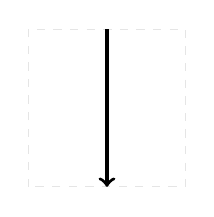
\begin{tikzpicture}[scale=2]
                \draw[dashed,white!90!black] (0,0) rectangle (1,1);
                \draw[very thick,->] (0.5,1) -- (0.5,0);
            \end{tikzpicture}
        }
    \end{choices}
    \end{multicols}
\end{question}
}


%% Section June1996
%%--------------------
\element{nysed}{
\begin{question}{June1995-Q10}
    A \SI{1.0e2}{\kilo\gram} box rests on the bed of a truck that is accelerating at \SI{2.0}{\meter\per\second\squared}.
    What is the magnitude of the force of friction on the box as it moves with the truck without slipping?
    \begin{multicols}{2}
    \begin{choices}
        \wrongchoice{\SI{1.0e3}{\newton}}
      \correctchoice{\SI{2.0e2}{\newton}}
        \wrongchoice{\SI{5.0e2}{\newton}}
        \wrongchoice{\SI{0.0}{\newton}}
    \end{choices}
    \end{multicols}
\end{question}
}

\element{nysed}{
\begin{question}{June1996-Q16}
    A horizontal force is used to pull a \SI{5.0}{\kilo\gram} cart at a constant speed of \SI{5.0}{\meter\per\second} across the floor,
        as shown in the diagram below.
    \begin{center}
    \begin{tikzpicture}
        %% Force 1
        \draw[thick,->] (0,0.5) -- (-4,0.5)
            node[above right] {$F_1=\SI{12}{\newton}$};
        %% Force 2
        \draw[thick,->] (2,0.5) -- (2.667,0.5);
        \node[anchor=south west] at (2,0.5) {$F_2=\SI{2}{\newton}$};
        %% Block
        \draw[thick] (0,0) rectangle (2,1);
        \node[anchor=center] at (1,0.5) {Block};
        %% Floor
        \draw[thick] (-3,0) -- (3,0);
        \node[anchor=north,minimum width=6cm,pattern=north east lines] at (0,0) {};
        \node[anchor=north] at (0,-0.15) {Frictionless surface};
    \end{tikzpicture}
    \end{center}
    If the force of friction that the cart and the floor is \SI{10}{\newton},
        the magnitude of the horizontal force along the handle of the cart is:
    \begin{multicols}{2}
    \begin{choices}
        \wrongchoice{\SI{5.0}{\newton}}
      \correctchoice{\SI{10}{\newton}}
        \wrongchoice{\SI{25}{\newton}}
        \wrongchoice{\SI{50}{\newton}}
    \end{choices}
    \end{multicols}
\end{question}
}


%% Section June1995
%%--------------------
\element{nysed}{
\begin{question}{June1995-Q12}
    A box decelerates as it moves to the right along a horizontal surface,
        as shown in the diagram.
    \begin{center}
    \begin{tikzpicture}
        %% ground
        \draw (-2,0) -- (4,0);
        \node[anchor=north,pattern=north east lines,minimum width=6cm] at (1,0) {};
        %% box
        \node[anchor=south,draw,fill=white!90!black,minimum width=2cm,minimum height=1cm] (A) at (0,0) {};
        \draw[thick,->] (A.east) -- ++(0:2) node[pos=0.5,anchor=south] {$v$};
    \end{tikzpicture}
    \end{center}
    Which vector best represents the force of friction on the box?
    \begin{multicols}{2}
    \begin{choices}
        \AMCboxDimensions{down=-0.8cm}
        \wrongchoice{
            \begin{tikzpicture}[scale=2]
                \draw[dashed,white!60!black] (0,0) rectangle (1,1);
                \draw[thick,->] (0.5,1) -- (0.5,0);
            \end{tikzpicture}
        }
        \wrongchoice{
            \begin{tikzpicture}[scale=2]
                \draw[dashed,white!60!black] (0,0) rectangle (1,1);
                \draw[thick,->] (0.5,0) -- (0.5,1);
            \end{tikzpicture}
        }
        \wrongchoice{
            \begin{tikzpicture}[scale=2]
                \draw[dashed,white!60!black] (0,0) rectangle (1,1);
                \draw[thick,->] (0,0.5) -- (1,0.5);
            \end{tikzpicture}
        }
        \correctchoice{
            \begin{tikzpicture}[scale=2]
                \draw[dashed,white!60!black] (0,0) rectangle (1,1);
                \draw[thick,->] (1,0.5) -- (0,0.5);
            \end{tikzpicture}
        }
    \end{choices}
    \end{multicols}
\end{question}
}


%% Section June1994
%%--------------------
\element{nysed}{
\begin{question}{June1994-Q05}
    A \SI{3.0}{\newton} force and a \SI{4.0}{\newton} force act concurrently on a point.
    In which diagram below would the orientation of these forces produce the greatest net force on the point?
    \begin{multicols}{2}
    \begin{choices}
        \AMCboxDimensions{down=-1cm}
        %% ANS is 1
        \correctchoice{
            \begin{tikzpicture}
                \draw[dashed,white!60!black] (-1.5,-1.5) rectangle (1.5,1.5);
                \draw[thick,->] (-1,-0.66) -- ++(0:2) node[pos=0.5,anchor=north] {\SI{4.0}{\newton}};
                \draw[thick,->] (-1,-0.66) -- ++(60:1.66) node[pos=1.0,anchor=south] {\SI{3.0}{\newton}};
            \end{tikzpicture}
        }
        \wrongchoice{
            \begin{tikzpicture}
                \draw[dashed,white!60!black] (-1.5,-1.5) rectangle (1.5,1.5);
                \draw[thick,->] (-1,-0.66) -- ++(0:2) node[pos=0.5,anchor=north] {\SI{4.0}{\newton}};
                \draw[thick,->] (-1,-0.66) -- ++(90:1.66) node[pos=0.5,anchor=west] {\SI{3.0}{\newton}};
            \end{tikzpicture}
        }
        \wrongchoice{
            \begin{tikzpicture}
                \draw[dashed,white!60!black] (-1.5,-1.5) rectangle (1.5,1.5);
                \draw[thick,->] (-0.66,-0.66) -- ++(0:2) node[pos=0.5,anchor=north] {\SI{4.0}{\newton}};
                \draw[thick,->] (-0.66,-0.66) -- ++(120:1.66) node[pos=0.5,anchor=south west] {\SI{3.0}{\newton}};
            \end{tikzpicture}
        }
        \wrongchoice{
            \begin{tikzpicture}
                \draw[dashed,white!60!black] (-1.5,-1.5) rectangle (1.5,1.5);
                \draw[thick,->] (-1,+0.66) -- ++(0:2) node[pos=0.5,anchor=south] {\SI{4.0}{\newton}};
                \draw[thick,->] (-1,+0.66) -- ++(270:1.66) node[pos=0.5,anchor=west] {\SI{3.0}{\newton}};
            \end{tikzpicture}
        }
    \end{choices}
    \end{multicols}
\end{question}
}

\element{nysed}{
\begin{question}{June1994-Q07}
    The diagram below represents a \SI{10}{\newton} block sliding down a \ang{30} incline at a constant speed.
    \begin{center}
    \begin{tikzpicture}
        %% ground
        \draw[thick] (-6,0) -- (1,0);
        %% incline
        \draw (0,0) -- (150:6) -- ++(270:{6*sin(30)}) -- cycle;
        \draw[<->,shorten >=1pt,shorten <=1pt] (180:1.33) arc (180:150:1.33) node[pos=0.5,anchor=east] {\ang{30}};
        %% block
        \node[draw,minimum size=1cm,anchor=south,rotate=-30] at (150:4) {\SI{10}{\newton}};
    \end{tikzpicture}
    \end{center}
    The force of friction on the block is approximately:
    \begin{multicols}{2}
    \begin{choices}
      \correctchoice{\SI{5.0}{\newton}}
        \wrongchoice{\SI{10}{\newton}}
        \wrongchoice{\SI{48}{\newton}}
        \wrongchoice{\SI{98}{\newton}}
    \end{choices}
    \end{multicols}
\end{question}
}

\element{nysed}{
\begin{question}{June1994-Q16}
    Which statement explains why a book resting on a table is in equilibrium?
    \begin{choices}
        \wrongchoice{There is a net force acting downward on the book}
        \wrongchoice{The weight of the book equals the weight of the table}
        \wrongchoice{The acceleration due to gravity is \SI{9.8}{\meter\per\second\squared} for both the book and the table.}
      \correctchoice{The weight of the book and the table's upward force on the book are equal in magnitude, but opposite in direction}
    \end{choices}
\end{question}
}



%% Section June1990
%%--------------------
\element{nysed}{
\begin{question}{June1990-Q13}
    The table below lists the coefficients of kinetic friction for four materials sliding over steel.
    \begin{center}
    \begin{tabular}{rc}
        \toprule
        Material & $\mu_k$ \\
        \midrule
        aluminum & 0.47 \\
        brass    & 0.44 \\
        copper   & 0.36 \\
        steel    & 0.57 \\
        \bottomrule
    \end{tabular}
    \end{center}
    A \SI{10}{\kilo\gram} block of each of the materials in the table is pulled horizontally across a steel floor at constant velocity.
    Which block would require the \emph{smallest} applied force to keep it moving at constant velocity?
    \begin{multicols}{2}
    \begin{choices}
        \wrongchoice{aluminum}
        \wrongchoice{brass}
      \correctchoice{copper}
        \wrongchoice{steel}
    \end{choices}
    \end{multicols}
\end{question}
}


%% Section June1989
%%--------------------
\element{nysed}{
\begin{question}{June1989-Q16}
    A cart rolls down an incline plane with constant speed as shown in the diagram.
    \begin{center}
    \begin{tikzpicture}
        %% ground and plane
        \draw (-6,0) -- (1,0);
        \node[minimum width=7cm,anchor=north,pattern=north east lines] at (-2.5,0) {};
        \draw (0,0) -- (150:{6/cos(30)});
        %% left Cart
        \path (60:0.2) ++ (150:{3/cos(30)}) node[draw,fill=white!90!black,minimum height=1cm,minimum width=1.5cm,anchor=south,rotate=-30] (L) {};
        %% options
        \draw[thick,->] (L) -- ++(-30:1.5) node[anchor=west] {$A$};
        \draw[thick,->] (L) -- ++(150:1.5) node[anchor=east] {$D$};
        \draw[thick,->] (L) -- ++(240:1.5) node[anchor=north east] {$C$};
        \draw[thick,->] (L) -- ++(270:1.5) node[anchor=north] {$B$};
        \draw[thick,->] (L.north west) ++ (60:1em) -- ++(330:1.5) node[pos=0.5,anchor=south,rotate=-30] {motion};
        %% wheels
        \draw[fill=white] (L.south west) ++(330:0.3) circle (0.2);
        \draw[fill=black] (L.south west) ++(330:0.3) circle (1pt);
        \draw[fill=white] (L.south east) ++(150:0.3) circle (0.2);
        \draw[fill=black] (L.south east) ++(150:0.3) circle (1pt);
    \end{tikzpicture}
    \end{center}
    Which arrow represents the direction of the frictional force?
    \begin{multicols}{4}
    \begin{choices}[o]
        \wrongchoice{$A$}
        \wrongchoice{$B$}
        \wrongchoice{$C$}
      \correctchoice{$D$}
    \end{choices}
    \end{multicols}
\end{question}
}


%% Section June1986
%%--------------------
\element{nysed}{
\begin{question}{June1986-Q06}
    A force of \SI{100}{\newton} is applied to an object at an angle of \ang{30} from the horizontal as shown in the diagram below.
    \begin{center}
    \begin{tikzpicture}
        %% ground
        \draw (-3,0) -- (3,0);
        \node[anchor=north,minimum width=6cm,pattern=north east lines] at (0,0) {};
        %% object
        \node[anchor=south,draw,minimum size=1.5cm] (A) at (-1.5,0) {Object};
        \draw[dashed] (A.east) -- ++(0:2);
        \draw[thick,-latex] (A.east) -- ++(30:3) node[anchor=south east,rotate=30] {\SI{100}{\newton}};
        \draw[<->,shorten >=1pt,shorten <=1pt] (A.east) ++(0:1) arc(0:30:1) node[pos=0.5,anchor=west] {\ang{30}};
    \end{tikzpicture}
    \end{center}
    What is the magnitude of the vertical component of this force?
    \begin{multicols}{2}
    \begin{choices}
        \wrongchoice{\SI{0.0}{\newton}}
      \correctchoice{\SI{50.0}{\newton}}
        \wrongchoice{\SI{87.7}{\newton}}
        \wrongchoice{\SI{100}{\newton}}
    \end{choices}
    \end{multicols}
\end{question}
}

\element{nysed}{
\begin{question}{June1986-Q17}
    Block $A$ is pulled with constant velocity up an incline as shown in the diagram below.
    \begin{center}
    \begin{tikzpicture}
        %% Floor
        \draw (6,0) -- (-1,0);
        \node[anchor=north,minimum width=7cm,pattern=north east lines] at (+2.5,0) {};
        \draw (5,0) -- (0,0) -- (30:{5/cos(30)}) -- cycle;
        %% Mass
        \node[draw,fill=white!90!black,rectangle,rounded corners=1ex,minimum size=1cm,rotate=30,anchor=south] (A) at (30:3) {$A$};
        \node[draw,fill=white!90!black,rectangle,rounded corners=1ex,minimum size=1cm,anchor=north] (B) at (5.66,2) {};
        \draw[thick,-latex] (A.north east) ++(30:1ex) -- ++(30:1) node[pos=0.5,anchor=south,rotate=30] {$v$};
        %% Rope and Pully
        \draw[thick,fill=white!90!black] (5.33,{5.67*tan(30)}) circle (0.33);
        \draw[thick] (A.east) -- ++(30:{(5/cos(30))-3});
        \draw[thick] (B.north) -- ++(90:{(5.67*tan(30))-2});
        \draw[thick,fill=white] (5,{5*tan(30)}) -- ++(64:0.52) arc(154:-26:0.12) -- (5,2.33) -- cycle;
        \fill (5.33,{5.67*tan(30)}) circle (1.25pt);
    \end{tikzpicture}
    \end{center}
    Which arrow best represents the direction of the force of friction acting on block $A$?
    \begin{multicols}{2}
    \begin{choices}
        \AMCboxDimensions{down=-0.4cm}
        \wrongchoice{
            \begin{tikzpicture}[scale=0.5]
                \draw[dashed] (-1.5,-1.5) rectangle (1.5,1.5);
                \draw[thick,-latex] (0,0) -- (210:1.5) -- ++(30:3);
            \end{tikzpicture}
        }
        %% ANS is 2
        \correctchoice{
            \begin{tikzpicture}[scale=0.5]
                \draw[dashed] (-1.5,-1.5) rectangle (1.5,1.5);
                \draw[thick,-latex] (0,0) -- (30:1.5) -- ++(210:3);
            \end{tikzpicture}
        }
        \wrongchoice{
            \begin{tikzpicture}[scale=0.5]
                \draw[dashed] (-1.5,-1.5) rectangle (1.5,1.5);
                \draw[thick,-latex] (0,0) -- (120:1.5) -- ++(300:3);
            \end{tikzpicture}
        }
        \wrongchoice{
            \begin{tikzpicture}[scale=0.5]
                \draw[dashed] (-1.5,-1.5) rectangle (1.5,1.5);
                \draw[thick,-latex] (0,0) -- (300:1.5) -- ++(120:3);
            \end{tikzpicture}
        }
    \end{choices}
    \end{multicols}
\end{question}
}


%% Section June1985
%%--------------------
\element{nysed}{
\begin{question}{June1985-Q06}
    In the diagram below, the numbers 1,2,3, and 4 represent possible directions in which a force could be applied to a cart.
    \begin{center}
    \begin{tikzpicture}
        %% Cart
        \node[minimum width=2.5cm,minimum height=1cm,draw,fill=white!90!black] (A) at (0,0) {};
        %% Wheels
        \draw[fill=white] (A.south west) ++ (+0.4,0) circle (0.3);
        \draw[fill=black] (A.south west) ++ (+0.4,0) circle (1.5pt);
        \draw[fill=white] (A.south east) ++ (-0.4,0) circle (0.3);
        \draw[fill=black] (A.south east) ++ (-0.4,0) circle (1.5pt);
        %% options
        \foreach \x/\y in {90/A,120/B,150/C,180/D}
            \draw[thick,-latex,shorten <=1pt] (A.north west) -- ++(\x:2) node[anchor=center,shift={(\x:0.5em)}] {$\y$};
    \end{tikzpicture}
    \end{center}
    If the force applied in each direction has the same magnitude,
        in which direction will the vertical component of the force be the \emph{least}?
    \begin{multicols}{4}
    \begin{choices}[o]
        \wrongchoice{$A$}
        \wrongchoice{$B$}
        \wrongchoice{$C$}
      \correctchoice{$D$}
    \end{choices}
    \end{multicols}
\end{question}
}

\element{nysed}{
\begin{question}{June1985-Q07}
    The diagram below represents two forces acting concurrently on an object.
    \begin{center}
    \begin{tikzpicture}
        \fill (0,0) circle (1.5pt);
        \draw (0,1em) -- (1em,1em) -- (1em,0);
        \draw[thick,-latex] (0,0) -- (0:4) node[pos=0.5,anchor=south] {\SI{40}{\newton}};
        \draw[thick,-latex] (0,0) -- (90:2) node[pos=0.5,anchor=south,rotate=90] {\SI{20}{\newton}};
    \end{tikzpicture}
    \end{center}
    The magnitude of the resultant force is closest to:
    \begin{multicols}{2}
    \begin{choices}
        \wrongchoice{\SI{20}{\newton}}
        \wrongchoice{\SI{40}{\newton}}
      \correctchoice{\SI{45}{\newton}}
        \wrongchoice{\SI{60}{\newton}}
    \end{choices}
    \end{multicols}
\end{question}
}

\element{nysed}{
\begin{question}{June1985-Q55}
    As the vector sum of all the forces acting on an object increases,
        the acceleration of the object:
    \begin{choices}
        \wrongchoice{decreases}
      \correctchoice{increases}
        \wrongchoice{remains the same}
    \end{choices}
\end{question}
}


\endinput


